\chapter{Clustering}\label{chap:clustering}

To better understand the data and to help with the task of finding anomalies, we will be using clustering techniques. These techniques are used to group data points that are similar to each other. The goal is to find groups of data points that are similar to each other, but different from the rest of the data. This is done by finding the distance between each data point and the rest of the data. The distance between two data points is calculated using a distance metric.

In this chapter, the clustering methods that were used will be briefly explained in section \ref{sec:clustering_methods}. Next, the dimensionality reduction methods used in some of the tests will be presented in section \ref{sec:dim_reduction}. 
% TODO

\section{Clustering Methods}\label{sec:clustering_methods}
Clustering is defined as the task of finding and then grouping the data values that are close to each other in some way. Because of this, clustering is not only a useful technique for data analysis but also for the task of anomaly detection, as abnormal samples tend to be far from the rest of the data. In this section, the clustering methods that were used in this work will be presented.

\subsection{K-Means}\label{sec:kmeans} 

The objective of K-means is to find a partition of the data into K clusters, where each data point belongs to the cluster with the nearest mean. The K-means algorithm is an iterative algorithm that starts by randomly assigning each data point to a cluster. Then, the mean of each cluster is calculated and the data points are reassigned to the cluster with the nearest mean. This process is repeated until the data points stop changing clusters. 

The number of divisions is defined by the $k$ parameter, which can be determined with the help of the following methods:

\begin{itemize}
    \item \textbf{Elbow Method:} The elbow method is a heuristic method that is used to find the optimal number of clusters. This method plots the sum of squared errors (SSE) for each value of $k$ and then finds the value of $k$ that has the "elbow" in the plot. This value of $k$ is considered to be the optimal number of clusters. This method presents some disadvantages, as it is not always clear where the "elbow" is, making it a subjective method. Also, the SSE is not a good measure of the quality of the clustering, as it is biased towards clusters with similar sizes.
    % TODO disadvantages
    \item \textbf{Silhouette Method:} The silhouette method is a method that is used to find the optimal number of clusters. This method calculates the silhouette coefficient for each data point, by evaluating the intra-cluster and inter-cluster distances. Scores for each point can range from -1 to 1, with lower values indicating that the data point is in the wrong cluster and higher values that it is in the correct cluster. The silhouette coefficient for each cluster is then calculated by averaging the silhouette coefficients of the data points in the cluster. Finally, the score for the entire dataset is calculated by averaging the coefficients from every cluster. The optimal number of clusters is the value of $k$ that has the highest silhouette coefficient.
\end{itemize}

K-means is advantageous when compared to other clustering methods because of its simplicity and the fact that it doesn't require any prior knowledge of the data. However, the disadvantages are that it is biased towards spherical clusters with similar sizes, is sensitive to the initial position of cluster centroids and requires the determination of the number of clusters beforehand.

\subsection{SOM}\label{sec:som}
This method is based on the idea of self-organizing maps, which are artificial neural networks used to find a low-dimensional representation of a high-dimensional space. It is usually employed to reduce the dimensions of the data to a map, but can also be used as a clustering method, as it groups similar data. 

The algorithm starts by randomly assigning each data point to a neuron in the map. Then, the weights of each neuron are updated to be closer to the data point that it represents. This process is repeated until the data points stop changing neurons. 

The advantage of this algorithm is that it can map high-dimensional input vectors to a low-dimensional space while preserving the original topology of the data. Unlike other clustering methods, which aren't able to provide good results for data with high dimensionality.\footnote{Self-Organizing Maps \url{https://sites.pitt.edu/~is2470pb/Spring05/FinalProjects/Group1a/tutorial/som.html}}

\subsection{Agglomerative Clustering}\label{sec:aglomerative}
Agglomerative clustering is a hierarchical clustering method that starts by assigning each data point to its own cluster. Then, the two clusters that are closest to each other are merged into a single cluster. This process is repeated until all the data points are in the same cluster. These are combined by comparing intra-cluster and inter-cluster distances. Distance between the clusters is calculated using a linkage function, and the distance between the data points in the clusters is calculated using a distance metric (normally the Euclidean distance). The size and shape of the clusters are directly influenced by these two parameters.

The number of clusters can be determined with the help of a dendogram plot. This plot shows the distance between the clusters as they are merged. Each leaf in the dendrogram represents a data point that is fused with a similar point into the same cluster as the height of the tree increases. The height of the fusion (on the vertical axis) represents the dissimilarity score between the two clusters. Higher fusions indicate that the clusters are more distinct. As a rule of thumb, the number of clusters can be determined by looking at the height of the fusion(s) that has the most distinct clusters (higher dissimilarity scores).\footnote{Agglomerative Clustering \url{https://www.datanovia.com/en/lessons/agglomerative-hierarchical-clustering/}}

One of the problems with this method is that there is no clear way to determine the number of clusters, as the dendrogram doesn't always produce clear divisions, making the process of choosing the number of clusters subjective.

\subsection{DBSCAN}\label{sec:dbscan}
This unsupervised clustering method was first introduced in Ester et al. \cite{dbscan}. It is a density-based clustering algorithm that is used to find clusters of data points that are close to each other. The algorithm assigns "core" labels to the points that have at least $minPts$ points within a distance $eps$ from them. Points that are reachable from a core point, but do not have at least $minPts$ points within a distance $eps$ from them, are assigned "border" labels. These are considered to be a part of the cluster formed by the core point.

The points that are not reachable from any core point are assigned "noise" labels and are considered to be outliers. Because of this, the algorithm provides a basic method for outlier detection.

The algorithm is advantageous because it doesn't require the determination of the number of clusters beforehand, as it can find clusters of any size and is also robust to the existence of outliers. Despite this, it is sensitive to the parameters $minPts$ and $eps$, with slight changes in these parameters having a significant impact on the results.

\section{Validity Measures\label{sec:validity_measures}}
As previously stated, one of the main difficulties in clustering is deciding the right number of clusters to ensure a clear division of the data. This is a subjective process that can be aided by the use of validity measures. These measures, often called indices, are used to evaluate the quality of the clustering and can be used to determine the optimal number of clusters. In this section, the validity measures that were used in this work will be presented.

Cluster validity indices can be divided into three categories: external, internal and relative. External validity indices are used to compare the results of the clustering with the ground truth (labels). On the other hand, internal validity indices serve to evaluate the quality of the clustering without the use of external information. Relative validity evaluates the clustering structure by varying different parameters of the algorithm, such as the number of clusters.

External validity criteria will not be considered for this study as there is no ground truth information available. Instead, internal and relative validity approaches will be used to evaluate the quality of the clustering. The internal validity indices that were used are the following:

\noindent\textbf{Silhouette Score (S).} This score is one of the most widely used to evaluate clustering goodness. It is also referred to as the mean Silhouette Coefficient for all clusters and is calculated with the mean intra-cluster distance and the mean nearest-cluster distance. Observations with a score close to 1 are well clustered, while observations with a score close to -1 are likely to be assigned to the wrong cluster. Scores around 0 indicate overlapping clusters.

\noindent\textbf{Calinski-Harabasz Index (CH).} This index is also known as the Variance Ratio Criterion. It is calculated by dividing the between-cluster or inter-cluster dispersion by the within-cluster or intra-cluster dispersion. The higher the value of the index, the better the clustering. Like the silhouette score, it evaluates the goodness of the clustering structure, with higher values indicating better clustering; but, contrary to the previous score, it has no reasonable bound and can take any value. Because of this, it is difficult to use this metric to compare clusterings generated with different methods.

\noindent\textbf{Davies-Bouldin Index (DB).} This index is calculated by taking the average similarity measure of each cluster with its most similar cluster. This is done by calculating intra-cluster dispersion for each cluster, $i$, followed by the separation measure of each cluster with every other cluster, $j$. Then the similarity of a cluster is obtained by dividing the sum of the intra-cluster dispersions of $i$ and $j$ by the distance between the centroids of the two. Next for each cluster, the maximum similarity measure is selected and the average of these values is calculated. Unlike the previous measures, the lower the value of the index, the better the clustering, as this indicates less similarity between clusters.

\section{Dimensionality Reduction}\label{sec:dim_reduction}
In Data Science and Machine Learning, dimensionality refers to the number of features of the dataset. The dimensionality of a dataset can be reduced by removing features that are not relevant to the problem at hand. This can be done by using feature selection methods, which are methods that select the most relevant features for the task at hand. However, this can also be done by using dimensionality reduction methods, which are methods that transform the data into a lower-dimensional space, while preserving the most important information.

These processes are useful in these contexts because they can reduce the computational cost of the algorithms, as well as the time needed to train the models. They can also improve the performance of the algorithms, as they can remove noise and irrelevant features from the data.

From the data analysis in Section \ref{sec:data_prelim_analysis}, it can be seen that each line, representing a distinct variable, has 640 abscissas which translate to the same number of features. This is an extremely high number of features that can be problematic for some algorithms, as the features are not all equally relevant to the problem at hand. Therefore, it is important to reduce the dimensionality of the dataset, so that the algorithms can be trained more efficiently and efficiently. 

In this case, variables with the same repeating values with be considered less important and be discarded by the dimensionality reduction algorithm, giving more emphasis on other variables that have more variation. This will be the case for the $R$ variable which is almost constant throughout every line measurement and thus provides almost no meaningful information.

For this work, we will be using the following dimensionality reduction methods:

\begin{itemize}
    \item \textbf{PCA:} Principal Component Analysis is a linear dimensionality reduction method that uses Singular Value Decomposition to project the data into a lower-dimensional space. It is advantageous because it is fast and efficient, but it is also sensitive to outliers.
    \item \textbf{t-SNE:} t-Distributed Stochastic Neighbor Embedding is a non-linear dimensionality reduction method that is based on the idea that similar data points should be close to each other in the lower-dimensional space. It is advantageous because it can preserve the topology of the data, but it is also computationally expensive.
\end{itemize}
% TODO falar da distributição dos dados para cada variável e como quaase todas as linhas de R têm sempre o mesmo valor no início e no fim

\section{Experiments}\label{sec:clustering_experiments}
After the identification of the most common clustering and dimensionality reduction methods, the next step is to apply them to the dataset and evaluate their performance. This section will describe the experiments that were carried out to try to better understand the dataset. 

In every experiment, the data was scaled with the QuantileTransformer module from the \textit{sklearn} \cite{scikit-learn} library. This module transforms the data to follow a uniform or a normal distribution. This is done to avoid the influence of outliers in the results of the clustering algorithms. This scaling method was also chosen out of consistency, as it will be later used to scale the data for the machine learning algorithms. Additionally, every algorithm and method that depends on random initialization was set to the same seed to ensure reproducibility.

\subsection{Time Series KMeans}\label{sec:time_series_methods}
The first method to be tested was the \textit{TimeSeriesKmeans}\footnote{TimeSeriesKMeans \url{https://tslearn.readthedocs.io/en/stable/gen_modules/clustering/tslearn.clustering.TimeSeriesKMeans.html}} clustering algorithm from \textit{tslearn} \cite{tslearn}. As the name indicates, this algorithm is a variation of the K-means algorithm that is used for time series data. It is advantageous as it can cluster time series data without the need to transform it into a vector, which can be problematic because it can lead to the loss of information. Despite this, the method is still based on the K-Means algorithm presented in Section \ref{sec:kmeans} and presents the same disadvantages as the original algorithm. 

Clustering was conducted first on the magnetic field ($B$) and then on the flux tube inclination ($\alpha$) variable. For each one an elbow test was conducted to try and determine the most appropriate number of clusters. 

\begin{figure}[h]
    \caption{TimeSeriesKMeans Elbow Tests}
    \begin{subfigure}[h]{0.48\textwidth}
        \centering
        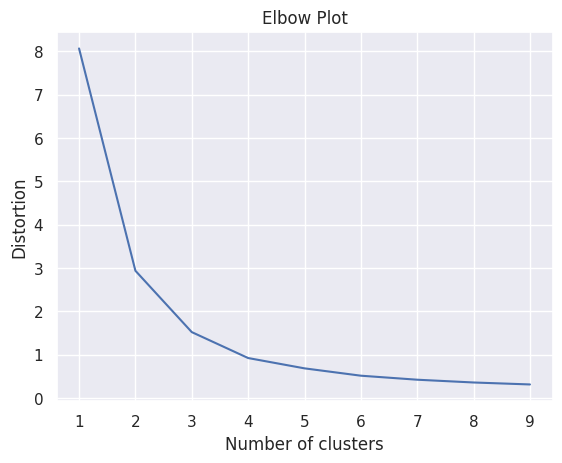
\includegraphics[width=\textwidth]{figures/tskmeans_elbow_b.png}
        \caption{Magnetic Field ($B$).}
        \label{fig:elbow_b}
    \end{subfigure}
    \hfill
    \begin{subfigure}[h]{0.48\textwidth}
        \centering
        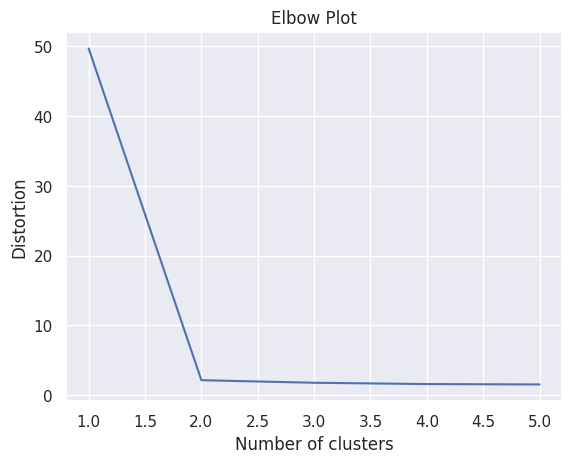
\includegraphics[width=\textwidth]{figures/tskmeans_elbow_alpha.png}
        \caption{Flux-tube inclination ($\alpha$).}
        \label{fig:elbow_alpha}
    \end{subfigure}
\end{figure}

\begin{table}[h]
    \caption[Validity Scores for TimeSeriesKmeans]{Validity metrics for different TimeSeriesKMeans models obtained by varying the number of clusters.}
    \begin{subtable}[h]{0.48\textwidth}
        \centering
        \begin{tabular}{@{}cccc@{}}
            \toprule
            \textbf{K} & \textbf{S score} & \textbf{DB} & \textbf{CH} \\ \midrule
            2          & 0.524               & 0.669                   & 20376                  \\
            3          & 0.511               & 0.628                   & 25585                  \\
            4          & 0.498               & 0.606                   & 30677                  \\
            5          & 0.458               & 0.648                   & 31995                  \\
            6          & 0.449               & 0.671                   & 34394                  \\
            7          & 0.431               & 0.695                   & 35462                  \\
            8          & 0.422               & 0.712                   & 36070                  \\
            9          & 0.403               & 0.738                   & 36368                  \\ \bottomrule
        \end{tabular}
        \caption{Magnetic Field ($B$)}
        \label{tab:tskmeans_b}
    \end{subtable}
    \hfill
    \begin{subtable}[h]{0.48\textwidth}
        \centering
        \begin{tabular}{@{}cccc@{}}
            \toprule
            \textbf{K} & \textbf{S score} & \textbf{DB} & \textbf{CH} \\ \midrule
            2          & 0.865               & 0.190                   & 263222                 \\
            3          & 0.499               & 1.078                   & 160481                 \\
            4          & 0.493               & 1.089                   & 120114                 \\
            5          & 0.463               & 1.123                   & 93537                  \\
            6          & 0.480               & 1.104                   & 82431                  \\
            7          & 0.259               & 1.312                   & 82038                  \\
            8          & 0.257               & 1.306                   & 76633                  \\
            9          & 0.252               & 1.374                   & 70313                  \\ \bottomrule
            \end{tabular}
        \caption{Flux-tube inclination ($\alpha$)}
        \label{tab:tskmeans_alpha}
    \end{subtable}
\end{table}


The elbow test for the magnetic field variable can be seen in Figure \ref{fig:elbow_b}. From this plot, it can be seen that the elbow is at $k=4$, which indicates that the optimal number of clusters is 4. However, this is not a clear elbow, as the curve is not smooth and the elbow is not very pronounced. This indicates that the optimal number of clusters is not very clear and that the results might not be very good.

To get a more precise number of clusters the validity metrics discussed in Section \ref{sec:validity_measures} were calculated for different KMeans models obtained by varying the number of clusters. The results of these tests can be seen in Table \ref{tab:tskmeans_b}. From the first three entries, it can be seen that the highest silhouette score is obtained with $K=2$, but the lowest Davies-Bouldin index is obtained with $k=4$, which also has the highest Calinski-Harabasz index of the three. This can serve as a possible indication that the correct number of clusters for this variable is 4.

Following the same procedure as for the magnetic field, an elbow test was conducted on the flux tube inclination variable, $\alpha$. The results of this test can be seen in Figure \ref{fig:elbow_alpha}. In contrast with the results of the previous test, this elbow is much clearer, with the elbow being at $k=2$. This indicates that the optimal number of clusters is 2.

The validity metrics (table \ref{tab:tskmeans_alpha}) also provide a clear indication that the correct number of clusters for this variable is 2, with the highest Silhouette and Calinski-Harabasz scores being obtained with $k=2$. The Davies-Bouldin index is also the lowest for this value.


\subsection{SOM}\label{sec:som_experiments}
Following the experiments with TimeSeriesKmeans, the SOM algorithm was tested, which is also seen as a useful method for clustering high-dimension data. A Python implementation of the algorithm \cite{vettigliminisom} was tested on the same variables as the previous algorithm, $B$ and $\alpha$. Unlike KMeans, this algorithm does not have any tests to visually determine the number of clusters. Because of this, the number of clusters was determined by trial and error, by varying the number of clusters and evaluating the results of the validity metrics (table \ref{tab:validity_som}). The first two columns of each subtable indicate the $x$ and $y$ dimensions of the SOM map used for the clustering task. The number of clusters is obtained by multiplying these two values.

\begin{table}[h]
    \caption[Validity Scores for SOM]{Validity metrics for different SOM models obtained by varying sizes of the maps ($x$ and $y$ variables).}\label{tab:validity_som}
    \begin{subtable}[h]{0.48\textwidth}
        \centering
        \begin{tabular}{@{}ccccc@{}}
            \toprule
            \textbf{x} & \textbf{y} & \textbf{S score} & \textbf{DB} & \textbf{CH} \\ \midrule
            2          & 2          & 0.500            & 0.602       & 30962   \\
            2          & 3          & 0.281            & 5.228       & 3429    \\
            3          & 2          & 0.454            & 0.660       & 35001   \\
            3          & 3          & 0.407            & 0.727       & 37133   \\ \bottomrule
            \end{tabular}
        \caption{Magnetic Field ($B$)}
        \label{tab:som_b}
    \end{subtable}
    \hfill
    \begin{subtable}[h]{0.48\textwidth}
        \centering
        \begin{tabular}{@{}ccccc@{}}
            \toprule
            \textbf{x} & \textbf{y} & \textbf{S score} & \textbf{DB} & \textbf{CH} \\ \midrule
            2          & 2          & 0.269            & 1.479       & 122195 \\
            2          & 3          & 0.004            & 1.325       & 5254    \\
            3          & 2          & 0.269            & 1.326       & 89759   \\
            3          & 3          & 0.231            & 1.426       & 66878   \\ \bottomrule
            \end{tabular}
        \caption{Flux-tube inclination ($\alpha$)}
        \label{tab:som_alpha}
    \end{subtable}
\end{table}

From looking at the results of the validity metrics for the magnetic field variable (table \ref{tab:som_b}), it can be concluded that the highest Silhouette score and DB index are obtained with $x=2$ and $y=2$, which translate to 4 clusters. For a map size of $x=2$ and $y=3$, the algorithm completely failed to generate a proper separation. The Calinski-Harabasz index is the highest for $x=3$ and $y=3$, which translates to 9 clusters. However, this is not a clear indication that this is the correct number of clusters, as the DB index is higher than the first clustering.

The results of the validity metrics for the flux tube inclination variable (table \ref{tab:som_alpha}) are even less clear than the previous ones. The highest Silhouette score is obtained with the first and third models. The best CH index was by far the first one. The DB index is very high for every model that was generated, which indicates that clustering in this variable may not be a good idea.

Overall the results from this experiment indicate that the SOM algorithm is not a good choice for clustering this dataset, as it is not able to generate a clear separation between the clusters. This is especially true for the flux tube inclination variable, where the algorithm completely failed to generate a proper separation. The only variable where the algorithm was able to generate a somewhat clear separation was the magnetic field with a map of 2x2 neurons.


\subsection{PCA Clustering Approach}\label{sec:pca_clustering}
The next approach that was tested was to apply PCA to the dataset and then apply the clustering algorithms to the reduced dataset. This approach was tested on the magnetic field variable, $B[G]$, the flux tube inclination, $\alpha [deg]$, and lastly on a combination of all the input variables. 

Tests were conducted to try and find the optimal number of components that would explain the dataset. This was done by analyzing the cumulative explained variance of PCA models with different \textit{n\_components}. For $B$ and $\alpha$ about 99\% of the variance was explained by just 2 components. As for the combined dataset, 98\% was explained by also 2 components. With this, it can be concluded that it is valid to reduce the dimensionality of this dataset to just two components. This is useful because it provides a simplified representation of the data while preserving most of the information. 

The representations for each of the approaches can be seen in Figure \ref{fig:pca_mag_2d}. Note that the representation generated for the flux-tube indication and the joint inputs are very similar. This indicates that the flux-tube inclination variable is the one that contributes the most to the PCA.

For the clustering part, the KMeans and the AgglomerativeClustering methods of the \textit{sklearn} library were applied to each of the representations to determine the correct number of clusters with the same methodology as in the previous sections. 

\begin{figure}[h]
    \caption[PCA applied to the different variables]{PCA applied to the different variables. (a) and (b) represent the PCAs of the magnetic field variable ($B[G]$) and the flux-tube inclination variable ($\alpha [deg]$), respectively; (c) is the PCA of all input variables combined.}
    \label{fig:pca_mag_2d}
    \begin{subfigure}[h]{0.329\textwidth}
        \centering
        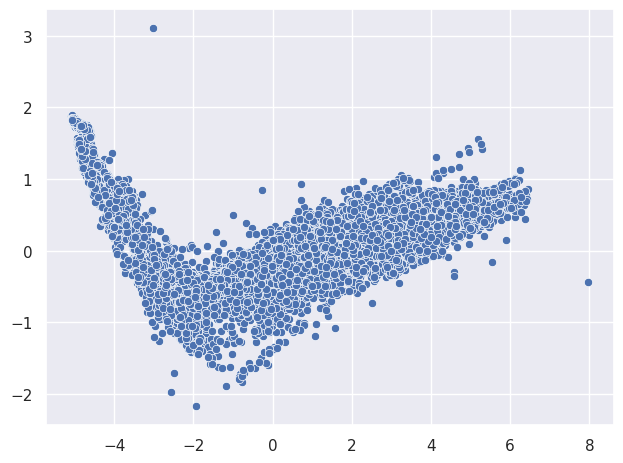
\includegraphics[width=\textwidth]{figures/mag_pca_2d.png}
        \caption{Magnetic Field ($B$).}
        \label{fig:pca_mag_2d}
    \end{subfigure}
    \hfill
    \begin{subfigure}[h]{0.329\textwidth}
        \centering
        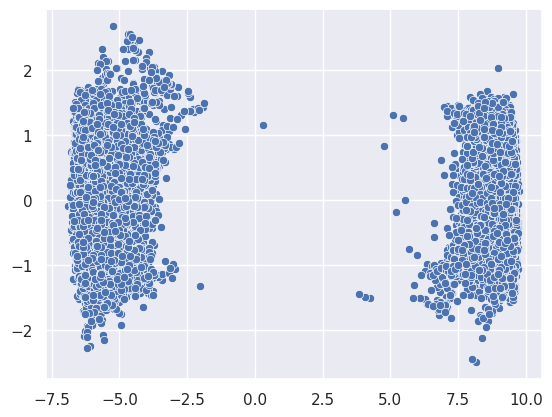
\includegraphics[width=\textwidth]{figures/alpha_pca_2d.png}
        \caption{Flux-tube inclination ($\alpha$).}
        \label{fig:pca_alpha_2d}
    \end{subfigure}
    \begin{subfigure}[h]{0.329\textwidth}
        \centering
        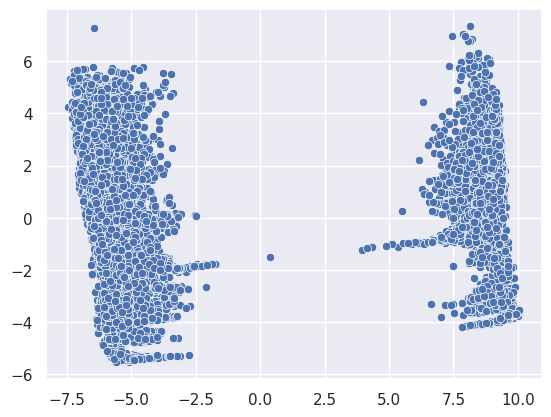
\includegraphics[width=\textwidth]{figures/pca_joint_2d.png}
        \caption{Joint Inputs ($R$, $B$ and $\alpha$).}
        \label{fig:pca_joint_2d}
    \end{subfigure}
\end{figure}

% \begin{figure}
%     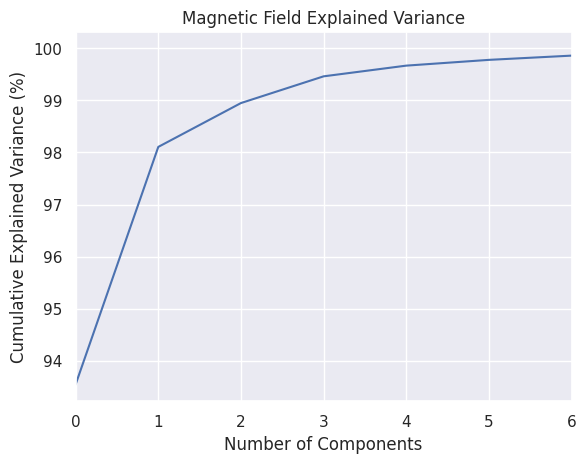
\includegraphics{figures/pca_mag_explained_variance.png}
%     \caption{Explained variance for the PCA of the magnetic field variable.}
% \end{figure}

\subsubsection{PCA of the Magnetic Field}\label{sec:pca_b}

The KMeans and the AgglomerativeClustering methods were applied to the PCA of the magnetic field variable. The results of the elbow tests for KMeans can be seen in Figure \ref{fig:pca_b_elbow}. From this plot, it can be seen that the elbow is at $k=4$, which is an indication that the optimal number of clusters might be 4. 

\begin{figure}
    \caption{KMeans Elbow test for the PCA of the magnetic field variable.}
    \label{fig:pca_b_elbow}
    \centering
    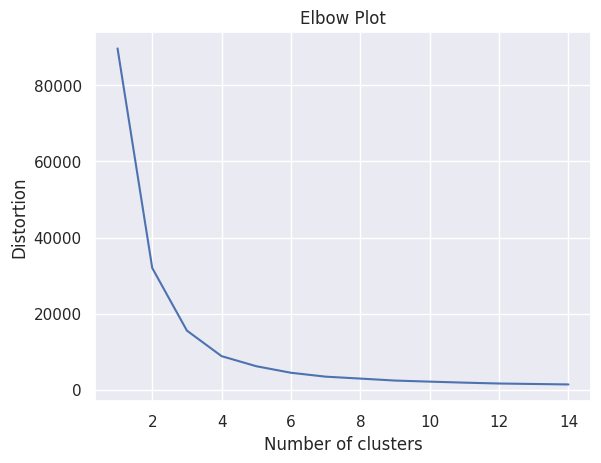
\includegraphics[width=0.6\textwidth]{figures/pca_mag_elbow_test.png}
\end{figure}

To get a more concrete outlook, the validity measures from the previous sections were calculated for each of the methods. The results of these tests can be seen in Table \ref{tab:pca_b}. For the KMeans algorithm, the highest Silhouette score is obtained with $K=2$, but the lowest Davies-Bouldin index is obtained with $K=4$, which also has the highest Calinski-Harabasz index of the first three results. This further confirms the results of the elbow test. 

The results of the Agglomerative method are not as clear as the previous ones. The highest silhouette score is also with $K=2$, but as in Kmeans, the lowest DB index was with $K=4$. In addition, the CH score is much higher for the model with 4 clusters than for the $K=2$ model.


% Please add the following required packages to your document preamble:
% \usepackage{booktabs}
\begin{table}[h]
    \caption[Validity metrics for PCA of the Magnetic Field]{Validity metrics obtained by different clustering methods on the PCA of the magnetic field variable. Various models were created for each method by varying the number of clusters, $K$.}\label{tab:pca_b}
    \begin{tabular}{@{}rrrrccc@{}}
        \cmidrule(l){2-7}
    \multicolumn{1}{c}{\textbf{}}   & \multicolumn{3}{c}{\textbf{KMeans}}                                                                       & \multicolumn{3}{c}{\textbf{Agglomerative}}   \\ \midrule
    \multicolumn{1}{c|}{\textbf{K}} & \multicolumn{1}{c}{\textbf{S score}} & \multicolumn{1}{c}{\textbf{DB}} & \multicolumn{1}{c|}{\textbf{CH}} & \textbf{S score} & \textbf{DB} & \textbf{CH} \\ \midrule
    \multicolumn{1}{r|}{2}          & 0.538                                & 0.645                           & \multicolumn{1}{r|}{21224}   & 0.507            & 0.669       & 17899   \\
    \multicolumn{1}{r|}{3}          & 0.534                                & 0.586                           & \multicolumn{1}{r|}{28086}   & 0.496            & 0.622       & 23868   \\
    \multicolumn{1}{r|}{4}          & 0.531                                & 0.549                           & \multicolumn{1}{r|}{35942}   & 0.502            & 0.550       & 30612   \\
    \multicolumn{1}{r|}{5}          & 0.502                                & 0.579                           & \multicolumn{1}{r|}{39762}   & 0.484            & 0.593       & 37737   \\
    \multicolumn{1}{r|}{6}          & 0.494                                & 0.592                           & \multicolumn{1}{r|}{44986}   & 0.477            & 0.585       & 40121   \\
    \multicolumn{1}{r|}{7}          & 0.486                                & 0.600                           & \multicolumn{1}{r|}{49233}   & 0.460            & 0.598       & 44158   \\
    \multicolumn{1}{r|}{8}          & 0.454                                & 0.637                           & \multicolumn{1}{r|}{49757}   & 0.436            & 0.638       & 45487   \\
    \multicolumn{1}{r|}{9}          & 0.457                                & 0.636                           & \multicolumn{1}{r|}{53265}   & 0.427            & 0.630       & 47528   \\ \bottomrule
    \end{tabular}
    \end{table}

With the consensus of both clustering methods, it can be concluded that the optimal number of clusters for the PCA of the magnetic field variable is 4. Interestingly, this is the same number of clusters that were obtained with the TimeSeriesKMeans algorithm in Section \ref{sec:time_series_methods} and the SOM algorithm in Section \ref{sec:som_experiments} for the magnetic field.

\subsubsection{PCA of the Flux-tube Inclination}\label{sec:pca_a}
Following the same procedure as in the previous approach, an elbow test was conducted for the KMeans model of the PCA of the flux-tube inclination variable. The results of this test can be seen in Figure \ref{fig:pca_a_elbow}. The plot indicates that the most appropriate number of clusters is 2.


\begin{figure}[h]
    \caption{KMeans Elbow test for the PCA of the flux-tube inclination variable.}
    \label{fig:pca_a_elbow}
    \centering
    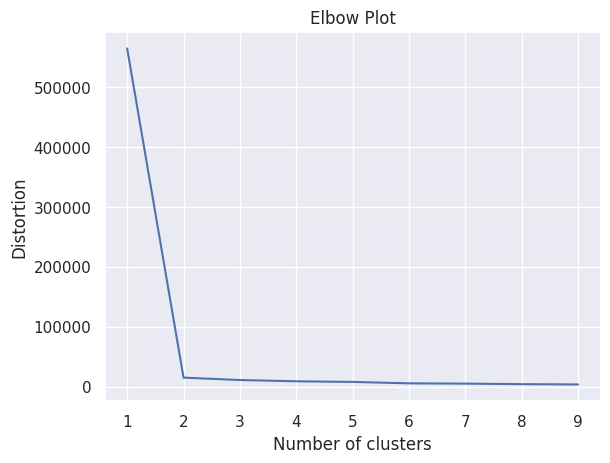
\includegraphics[width=0.6\textwidth]{figures/pca_alpha_elbow_test.png}
\end{figure}

These results are further corroborated by the validity metrics in Table \ref{tab:pca_a}. The highest Silhouette score and DB index are obtained with $K=2$, which also has the highest Calinski-Harabasz index of all the results. This indicates that the optimal number of clusters is 2, for both of the tested methods. This division occurs because the $\alpha$ variable may take negative or positive values.

\begin{table}[h]
    \caption[Validity metrics for PCA of the Flux-tube Inclination]{Validity metrics obtained by different clustering methods on the PCA of the flux-tube inclination variable. Various models were created for each method by varying the number of clusters, $K$.}\label{tab:pca_a}
    \begin{tabular}{@{}cccc|ccc@{}}
    \cmidrule(l){2-7}
    \multicolumn{1}{l}{}            & \multicolumn{3}{c|}{\textbf{KMeans}}         & \multicolumn{3}{c}{\textbf{Agglomerative}}   \\ \midrule
    \multicolumn{1}{c|}{\textbf{K}} & \textbf{S score} & \textbf{DB} & \textbf{CH} & \textbf{S score} & \textbf{DB} & \textbf{CH} \\ \midrule
    \multicolumn{1}{c|}{2}          & 0.898            & 0.145       & 428761  & 0.898            & 0.145       & 428761  \\
    \multicolumn{1}{c|}{3}          & 0.586            & 0.757       & 294424  & 0.574            & 0.782       & 287595  \\
    \multicolumn{1}{c|}{4}          & 0.593            & 0.662       & 243422  & 0.378            & 1.022       & 239082  \\
    \multicolumn{1}{c|}{5}          & 0.583            & 0.713       & 207238  & 0.354            & 0.955       & 219099  \\
    \multicolumn{1}{c|}{6}          & 0.400            & 0.887       & 237197  & 0.359            & 0.924       & 215351  \\
    \multicolumn{1}{c|}{7}          & 0.392            & 0.917       & 216689  & 0.360            & 0.900       & 211272  \\
    \multicolumn{1}{c|}{8}          & 0.391            & 0.875       & 225758  & 0.338            & 0.906       & 199083  \\
    \multicolumn{1}{c|}{9}          & 0.381            & 0.901       & 223637  & 0.336            & 0.890       & 189224  \\ \bottomrule
    \end{tabular}
    \end{table}

\subsubsection{PCA of the Joint Inputs}\label{sec:pca_joint}
In this next approach, the PCA was applied to the joint inputs, $R$, $B$ and $\alpha$. The results of the elbow test for the KMeans algorithm can be seen in Figure \ref{fig:pca_joint_elbow}. It is difficult to determine the optimal number of clusters from this plot. Possible "elbows" include the ones at $K=3$ and $K=6$.

\begin{figure}[h]
    \caption{KMeans Elbow test for the PCA of the joint inputs.}
    \label{fig:pca_joint_elbow}
    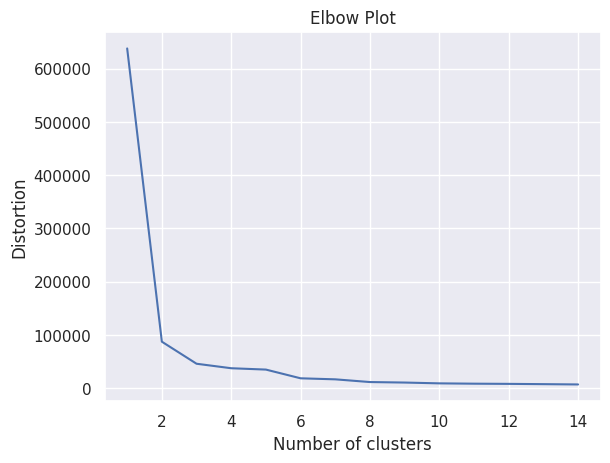
\includegraphics[width=0.6\textwidth]{figures/pca_joint_elbow_test.png}
\end{figure}

To draw better conclusions, the validity metrics were calculated for each of the methods. The results of these tests can be seen in Table \ref{tab:pca_joint}. For the KMeans algorithm, the highest Silhouette score and DB index are from $K=2$. This conflicts with the results of the elbow test, which indicated that the optimal number of clusters was 3 or 6. The highest CH index of the three is with $K=6$, but this model has the worst Silhouette and DB scores. At first glance, the optimal number of clusters would be 2 for the KMeans algorithm.

Next, for the Agglomerative method, the best silhouette score is from $K=2$ with the same results as the previous method. This is because both algorithms generate the same clear division of the dataset into two clusters that can easily be construed from Fig. \ref{fig:pca_joint_2d}. The remaining validity metrics are also very similar to the ones obtained with the KMeans algorithm. However, the clusters, generated by the Agglomerative method for $K=3$ had a smaller CH score than the ones for $K=2$. This might indicate that the best number of clusters for this method is 2.


\begin{table}[h]
    \caption[Validity metrics for PCA of the Joint Inputs]{Validity metrics obtained by different clustering methods on the PCA of the joint inputs. Various models were created for each method by varying the number of clusters, $K$.}\label{tab:pca_joint}
    \begin{tabular}{@{}lrcc|ccc@{}}
    \cmidrule(l){2-7}
    \textbf{}                       & \multicolumn{3}{c|}{\textbf{KMeans}}         & \multicolumn{3}{c}{\textbf{Agglomerative}}   \\ \midrule
    \multicolumn{1}{l|}{\textbf{K}} & \textbf{S score} & \textbf{DB} & \textbf{CH} & \textbf{S score} & \textbf{DB} & \textbf{CH} \\ \midrule
    \multicolumn{1}{l|}{2}          & 0.777            & 0.326       & 74261       & 0.777            & 0.326       & 74261       \\
    \multicolumn{1}{l|}{3}          & 0.647            & 0.494       & 75974       & 0.625            & 0.503       & 70716       \\
    \multicolumn{1}{l|}{4}          & 0.605            & 0.567       & 62966       & 0.544            & 0.564       & 72768       \\
    \multicolumn{1}{l|}{5}          & 0.553            & 0.698       & 50851       & 0.510            & 0.620       & 84236       \\
    \multicolumn{1}{l|}{6}          & 0.471            & 0.714       & 78768       & 0.464            & 0.704       & 86339       \\
    \multicolumn{1}{l|}{7}          & 0.465            & 0.747       & 73566       & 0.427            & 0.789       & 83135       \\
    \multicolumn{1}{l|}{8}          & 0.438            & 0.777       & 91850       & 0.396            & 0.819       & 82333       \\
    \multicolumn{1}{l|}{9}          & 0.435            & 0.786       & 87596       & 0.382            & 0.858       & 82094       \\ \bottomrule
    \end{tabular}
    \end{table}


\subsection{t-SNE Clustering Approach}\label{sec:tsne_clustering}
The last approach that was tested was to apply t-SNE to the dataset and then apply the clustering algorithms to the reduced dataset. As with the previous approach, this one was tested on the magnetic field variable, $B[G]$, the flux tube inclination, $\alpha [deg]$, and lastly on a combination of all the input variables. The embed 2D representations obtained from the t-SNE algorithm can be seen in Figure \ref{fig:tsne_2d}. Just by looking at the first two, it can be concluded that the clustering task will be more complicated than it was the PCA representations.

\begin{figure}[h]
    \caption{t-SNE applied to the different variables. (a) and (b) represent the t-SNE of the magnetic field variable ($B[G]$) and the flux-tube inclination variable ($\alpha [deg]$), respectively; (c) is the t-SNE of all input variables combined.}
    \label{fig:tsne_2d}
    \begin{subfigure}[h]{0.329\textwidth}
        \centering
        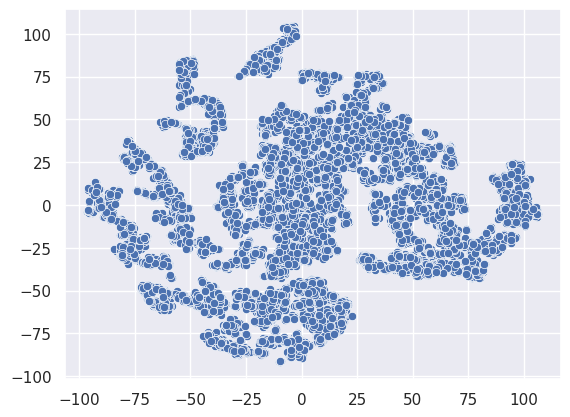
\includegraphics[width=\textwidth]{figures/tsne_mag_2d.png}
        \caption{Magnetic Field ($B$).}
        \label{fig:tsne_mag_2d}
    \end{subfigure}
    \hfill
    \begin{subfigure}[h]{0.329\textwidth}
        \centering
        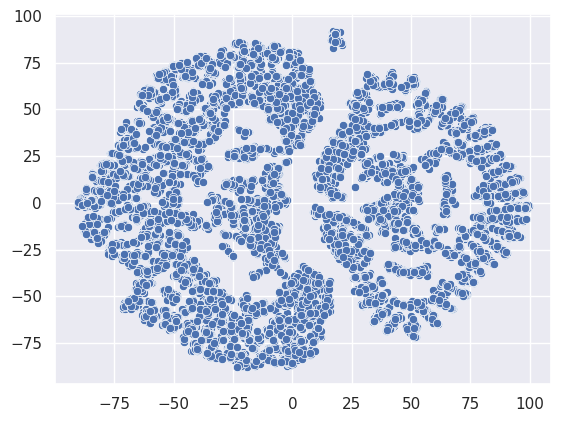
\includegraphics[width=\textwidth]{figures/tsne_alpha_2d.png}
        \caption{Flux-tube inclination ($\alpha$).}
        \label{fig:tsne_alpha_2d}
    \end{subfigure}
    \begin{subfigure}[h]{0.329\textwidth}
        \centering
        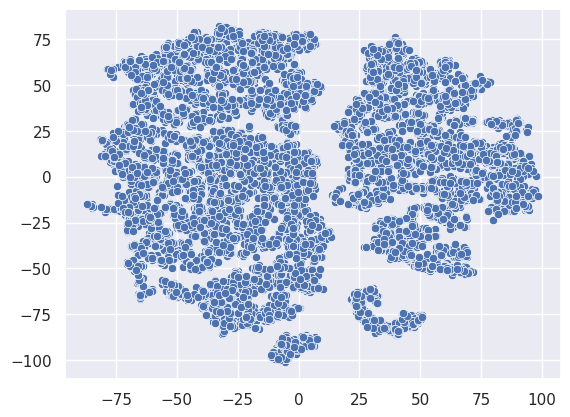
\includegraphics[width=\textwidth]{figures/tsne_joint_2d.png}
        \caption{Joint Inputs ($R$, $B$ and $\alpha$).}
        \label{fig:tsne_joint_2d}
    \end{subfigure}
\end{figure}

As in the previous section, each of the representations was subjected to the KMeans and Agglomerative clustering algorithms from the \textit{sklearn} library. The same validity metrics were calculated to determine what number of clusters would generate the best clustering.

\subsubsection{t-SNE of the Magnetic Field}\label{sec:tsne_b}
The elbow test for the magnetic field variable was inconclusive, as the elbow was not very clear. Possible values could be with 4 or 6 clusters. The highest Silhouette score is obtained with $K=2$, but the lowest Davies-Bouldin index is obtained with $K=4$, which also has the highest Calinski-Harabasz index of the first three results. 

% \begin{figure}
%     \caption{KMeans Elbow test for the t-SNE of the magnetic field variable.}
%     \label{fig:tsne_b_elbow}
%     \centering
%     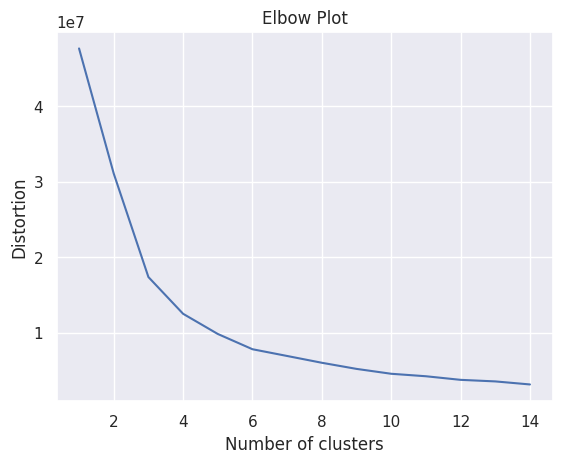
\includegraphics[width=0.6\textwidth]{figures/tsne_mag_elbow_test.png}
% \end{figure}

The validity metrics from Table \ref{tab:tsne_b} show a clear candidate for the KMeans method at $K=6$, which has the best scores of every other model. This disambiguates the results of the elbow test conducted previously. For the Agglomerative clustering method, the results aren't as pronounced. The best silhouette and DB scores were obtained for 6 clusters. Despite the CH index not being as higher as the rest, there is not much variation of this metric above 5 clusters. The results of this test indicate that the optimal number of clusters is 6 for both of the clustering methods.

\begin{table}[h]
    \caption[Validity metrics for t-SNE of the Magnetic Field]{Validity metrics obtained by different clustering methods on the t-SNE of the magnetic field variable. Various models were created for each method by varying the number of clusters, $K$.}\label{tab:tsne_b}
    \begin{tabular}{@{}rrrr|rrr@{}}
    \cmidrule(l){2-7}
    \multicolumn{1}{l}{}            & \multicolumn{3}{c|}{\textbf{KMeans}}         & \multicolumn{3}{c}{\textbf{Agglomerative}}   \\ \midrule
    \multicolumn{1}{r|}{\textbf{K}} & \textbf{S score} & \textbf{DB} & \textbf{CH} & \textbf{S score} & \textbf{DB} & \textbf{CH} \\ \midrule
    \multicolumn{1}{r|}{2}          & 0.323            & 1.265       & 6275.825    & 0.361            & 1.141       & 7475.524    \\
    \multicolumn{1}{r|}{3}          & 0.404            & 0.863       & 10259.411   & 0.349            & 0.883       & 7335.993    \\
    \multicolumn{1}{r|}{4}          & 0.409            & 0.838       & 11029.298   & 0.386            & 0.848       & 9553.107    \\
    \multicolumn{1}{r|}{5}          & 0.400            & 0.867       & 11319.886   & 0.387            & 0.853       & 10085.435   \\
    \multicolumn{1}{r|}{6}          & 0.424            & 0.756       & 12010.235   & 0.390            & 0.777       & 10395.708   \\
    \multicolumn{1}{r|}{7}          & 0.406            & 0.831       & 11557.172   & 0.358            & 0.842       & 10453.778   \\
    \multicolumn{1}{r|}{8}          & 0.402            & 0.798       & 11639.116   & 0.346            & 0.823       & 10364.565   \\
    \multicolumn{1}{r|}{9}          & 0.397            & 0.792       & 11998.942   & 0.357            & 0.827       & 10653.976   \\
    \multicolumn{1}{r|}{10}         & 0.403            & 0.785       & 12363.613   & 0.373            & 0.820       & 11237.525   \\ \bottomrule
    \end{tabular}
    \end{table}

\subsubsection{t-SNE of the Flux-tube Inclination}\label{sec:tsne_a}
In line with the results from the experiments on the magnetic field, the elbow test for the $\alpha$ variable is also difficult to interpret. The elbow is not clear enough to be able to reach an estimation.

The validity metrics in Table \ref{tab:tsne_a} also fail to indicate which is the optimal number of clusters for the KMeans algorithm. This can be because the algorithm is not suited to handle this representation, as it is very complex. The same can be said of the Agglomerative method, with all entries having very similar silhouette scores. A comparison of both DB and CH scores indicates that the number of clusters for both methods may be either 8 or 9, but there is no clear indication of which one is the best.

\begin{table}[h]
    \caption[Validity metrics for t-SNE of the Flux-tube Inclination]{Validity metrics obtained by different clustering methods on the t-SNE of the flux-tube inclination variable. Various models were created for each method by varying the number of clusters, $K$.}\label{tab:tsne_a}
    \begin{tabular}{@{}rrrr|rrr@{}}
    \cmidrule(l){2-7}
    \multicolumn{1}{l}{}            & \multicolumn{3}{c|}{\textbf{KMeans}}         & \multicolumn{3}{c}{\textbf{Agglomerative}}   \\ \midrule
    \multicolumn{1}{r|}{\textbf{K}} & \textbf{S score} & \textbf{DB} & \textbf{CH} & \textbf{S score} & \textbf{DB} & \textbf{CH} \\ \midrule
    \multicolumn{1}{r|}{2}          & 0.367            & 1.142       & 7613    & 0.343            & 1.112       & 6787    \\
    \multicolumn{1}{r|}{3}          & 0.410            & 0.803       & 10814   & 0.385            & 0.864       & 9815    \\
    \multicolumn{1}{r|}{4}          & 0.389            & 0.817       & 11185   & 0.350            & 0.887       & 8899    \\
    \multicolumn{1}{r|}{5}          & 0.382            & 0.877       & 11611   & 0.336            & 0.945       & 9269    \\
    \multicolumn{1}{r|}{6}          & 0.365            & 0.866       & 11396   & 0.366            & 0.867       & 9925    \\
    \multicolumn{1}{r|}{7}          & 0.396            & 0.779       & 12086   & 0.351            & 0.861       & 10223   \\
    \multicolumn{1}{r|}{8}          & 0.394            & 0.754       & 12678   & 0.338            & 0.799       & 10276   \\
    \multicolumn{1}{r|}{9}          & 0.395            & 0.776       & 12365   & 0.325            & 0.785       & 10429   \\
    \multicolumn{1}{r|}{10}         & 0.398            & 0.789       & 13223   & 0.341            & 0.853       & 10870   \\ \bottomrule
    \end{tabular}
    \end{table}

\subsubsection{t-SNE of the Joint Inputs}\label{sec:tsne_joint}
Contrary to the other two variables, the elbow test for the joint inputs is very clear (Fig.\ref{fig:tsne_joint_elbow}). The elbow is at $K=3$, which is an indication that the optimal number of clusters is 3. This is also corroborated by the validity metrics in Table \ref{tab:tsne_joint}. For the KMeans algorithm, the highest Silhouette score and DB index are with $K=2$, which also has the highest Calinski-Harabasz index of the first three results. Another possible division would be 7 clusters because of the similar silhouette and DB scores and a higher CH score. 

For the Agglomerative method, the most appropriate number of clusters is 3. Despite it having a worse DB index than on $K=4$, the silhouette and CH scores are better. This indicates that the optimal number of clusters is 3 for both of the clustering methods.

\begin{figure}[h]
    \caption{KMeans Elbow test for the t-SNE of the joint inputs.}
    \label{fig:tsne_joint_elbow}
    \centering
    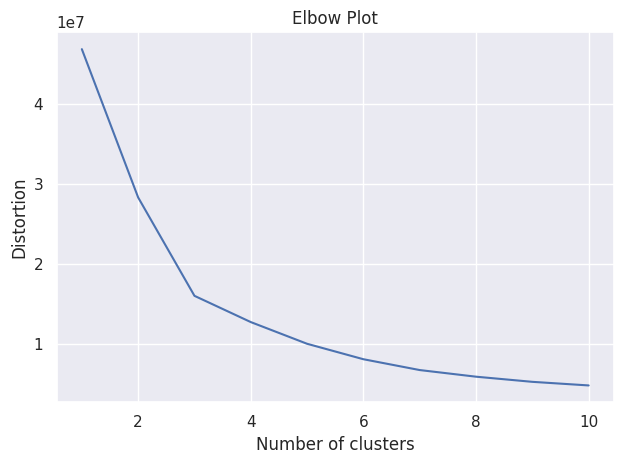
\includegraphics[width=0.6\textwidth]{figures/tsne_joint_elbow_test.png}
\end{figure}

% Please add the following required packages to your document preamble:
% \usepackage{booktabs}
\begin{table}[h]
    \caption[Validity metrics for t-SNE of the Joint Inputs]{Validity metrics obtained by different clustering methods on the t-SNE of the joint inputs. Various models were created for each method by varying the number of clusters, $K$.}\label{tab:tsne_joint}
    \begin{tabular}{@{}cccc|ccc@{}}
    \cmidrule(l){2-7}
                                    & \multicolumn{3}{c|}{\textbf{KMeans}}         & \multicolumn{3}{c}{\textbf{Agglomerative}}   \\ \midrule
    \multicolumn{1}{c|}{\textbf{K}} & \textbf{S score} & \textbf{DB} & \textbf{CH} & \textbf{S score} & \textbf{DB} & \textbf{CH} \\ \midrule
    \multicolumn{1}{c|}{2}          & 0.383            & 1.067       & 7701    & 0.328            & 1.068       & 5684    \\
    \multicolumn{1}{c|}{3}          & 0.430            & 0.791       & 11317   & 0.400            & 0.851       & 10083   \\
    \multicolumn{1}{c|}{4}          & 0.384            & 0.829       & 10493   & 0.370            & 0.790       & 9549    \\
    \multicolumn{1}{c|}{5}          & 0.370            & 0.918       & 10792   & 0.341            & 0.902       & 9797    \\
    \multicolumn{1}{c|}{6}          & 0.391            & 0.856       & 11249   & 0.330            & 0.972       & 9609    \\
    \multicolumn{1}{c|}{7}          & 0.399            & 0.798       & 11645   & 0.319            & 1.015       & 9572    \\
    \multicolumn{1}{c|}{8}          & 0.385            & 0.806       & 11612   & 0.328            & 0.941       & 9924    \\
    \multicolumn{1}{c|}{9}          & 0.377            & 0.850       & 11576   & 0.341            & 0.894       & 10287   \\
    \multicolumn{1}{c|}{10}         & 0.379            & 0.820       & 11369   & 0.337            & 0.888       & 10364   \\ \bottomrule
    \end{tabular}
    \end{table}

\section{ML Experiments}\label{sec:clustering_ml_experiments}
Following the mostly exploratory clustering experiments, the next step was to apply the clustering algorithms to the dataset and then use the resulting clusters to train different machine learning models. The objective of this experiment was to determine if models trained on clusters generated by different algorithms would be able to produce better predictions than models trained on the entire dataset. 

The reasoning behind this is that by grouping similar data points together, the models would be able to learn more specific patterns for each cluster. This is especially useful in this context as the data is very dispersed and the resulting models would converge to the mean of the dataset. % TODO referenciar Filipa

Due to the difficulty in selecting the most appropriate clustering, a grid-search-based approach was followed for this task. Several clusterings, $C$, were generated for each of the methods described in the previous sections, by varying the number of clusters, $K$. For consistency, the same clustering parameters from the previous experiments were used, also because they were chosen to be the most appropriate for each method and the dataset at hand.

Then, an ML model, $M_i$, was trained for each of the generated clusterings, $C_i$, was trained for each cluster, $C_{ij}$, where $i$ is the ith clustering and $j$ is the jth cluster of $C$. Each model, $M_i$, is trained with the same methodology as in \cite{barros_InitialConditionEstimation_}. Only this time instead of training a single model for the entire dataset, a model was trained for each cluster, $C_{ij}$. 

Following the methodology of \cite{barros_InitialConditionEstimation_}, the same validation files were extracted from the training dataset to later be used in the MULTI-VP tests. For each cluster, $C_{ij}$ a train test split of 85/15\% was done to obtain training and testing datasets. The training dataset was then used to train the models $M_{ij}$, and the testing dataset was later used to evaluate the models in terms of performance. In the next step, a hyper-tuning random search model from the \textit{keras} \cite{chollet2015keras} library was employed to find the best hyper-parameters for $M_{ij}$, based on the best test MSE loss. Finally, the best model was saved to later be used in the MULTI-VP experiments. 

All of the generated models were saved along with their statistics and the hyper-parameters used. The results of the MULTI-VP experiments can be seen in Section \ref{sec:clustering_ml_results}.

\subsection{Clustering ML Results}\label{sec:clustering_ml_results}
The results from the above mentioned experiments are presented in Table \ref{tab:clustering_ml_results}. Only the top 10 results based on MSE loss measured on the testing dataset are shown. The models are sorted based on the average MSE loss each experiment. This is obtained by averaging the MSE loss of each model, $M_{ij}$, for each cluster, $C_{ij}$, of each clustering, $C_i$. The models are sorted from lowest to highest average loss. The first column shows the model ID which briefly characterizes the model, the dimensionality reduction method, the variables used in the clustering, the clustering method, number of clusters, $K$, and the average loss and standard deviation of the models.


\begin{table}[h]
    \caption[Results of the Clustering ML Experiments]{Results of the Clustering ML Experiments. The table shows the 10 best models, based on the average MSE loss. The models are sorted by the average loss, from lowest to highest. The columns show the model ID, the dimensionality reduction method, the variables used, the clustering method, the number of clusters, $K$, the average loss of the models, the standard deviation of the loss and the sum of the loss and the standard deviation.}\label{tab:clustering_ml_results}
    \begin{tabular}{@{}cccccrr@{}}
    \toprule
    \textbf{Model ID}     & \textbf{Dim. Reduct.} & \textbf{Variable} & \textbf{Method} & \textbf{K} & \multicolumn{1}{c}{\textbf{Avg. Loss}} & \multicolumn{1}{c}{\textbf{std Loss}} \\ \midrule
    tsne\_agg\_2          & TSNE                  & Joint             & Agglom.         & 2          & 0.0108                                 & 0.0058                                \\
    pca\_kmeans\_2        & PCA                   & Joint             & KMeans          & 2          & 0.0113                                 & 0.0016                                \\
    pca\_kmeans\_3        & PCA                   & Joint             & KMeans          & 3          & 0.0119                                 & 0.0037                                \\
    pca\_agg\_2           & PCA                   & Joint             & Agglom.         & 2          & 0.0125                                 & 0.0012                                \\
    tsne\_kmeans\_mag\_3  & TSNE                  & Mag. Field        & KMeans          & 3          & 0.0125                                 & 0.0085                                \\
    tsne\_agg\_8          & TSNE                  & Joint             & Agglom.         & 8          & 0.0127                                 & 0.0077                                \\
    tsne\_agg\_alpha\_2   & TSNE                  & Alpha             & Agglom.         & 2          & 0.0129                                 & 0.0003                                \\
    pca\_kmeans\_alpha\_2 & PCA                   & Alpha             & KMeans          & 2          & 0.0130                                 & 0.0009                                \\
    tsne\_agg\_3          & TSNE                  & Joint             & Agglom.         & 3          & 0.0132                                 & 0.0093                                \\
    tsne\_agg\_mag\_3     & TSNE                  & Joint             & Agglom.         & 3          & 0.0132                                 & 0.0090                                \\ \bottomrule
    \end{tabular}
\end{table}


The experimental results (table \ref{tab:clustering_ml_results}) show that the best models were obtained with the clusterings of the TSNE joint inputs. These divisions were obtained by running the Agglomerative Clustering method with $K=2$. A closer look at the standard deviation of this model shows that it is the highest of the top 3 models, which indicates that there is a large disparity between the losses of both models. 

\begin{figure}
    \caption{Visualization of the clusters obtained with the TSNE of the joint inputs.}
    \label{fig:tsne_joint_kmeans_2}
    \centering
    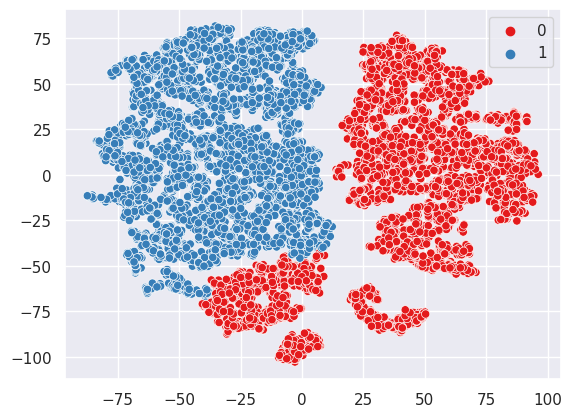
\includegraphics[width=0.6\textwidth]{figures/tsne_joint_kmeans_2.png}
\end{figure}

A more in-depth analysis of this outcome with the validity methods from table \ref{tab:tsne_joint} contradicts the results from this experiment. Despite it having the lowest loss of all the entries, the clustering quality was subpar for this instance. The inappropriate clustering of the dataset might be the reason for the high standard deviation of the models, as the data was not grouped correctly. A visualization of the clusters further corroborates this hypothesis. Figure \ref{fig:tsne_joint_kmeans_2} shows the clusters obtained with the TSNE of the joint inputs. It is clear that the clusters are not well defined and that the data is not grouped correctly. 

\begin{figure}[h]
    \caption[Top clustering results for the KMeans applied to the PCA of the joint inputs.]{Top clustering results for the KMeans applied to the PCA of the joint inputs. Clusters were obtained with the KMeans algorithm on the PCA of the joint inputs with $K=2$ on the left and $K=3$ on the right.}
    \label{fig:pca_joint_kmeans_results}
    \begin{subfigure}[h]{0.49\textwidth}
        \centering
        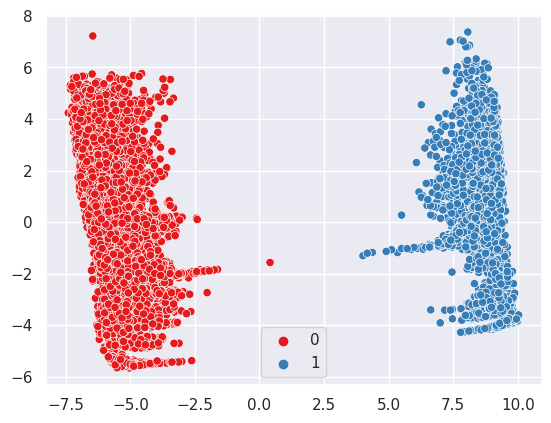
\includegraphics[width=\textwidth]{figures/pca_joint_kmeans_2.png}
        \caption{2 clusters}
        \label{fig:pca_joint_kmeans_2}
        % \label{fig:tsne_mag_2d}
    \end{subfigure}
    \hfill
    \begin{subfigure}[h]{0.49\textwidth}
        \centering
        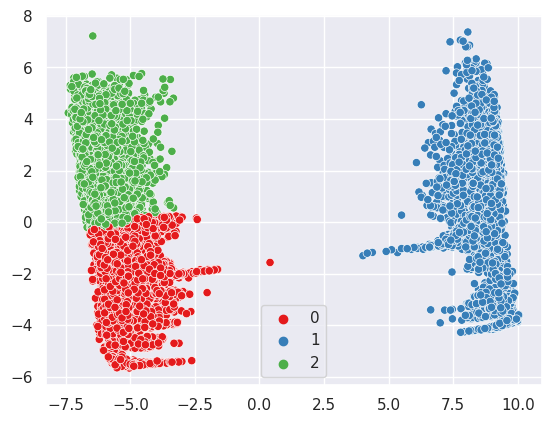
\includegraphics[width=\textwidth]{figures/pca_joint_kmeans_3.png}
        \caption{3 clusters}
        \label{fig:pca_joint_kmeans_3}
    \end{subfigure}
\end{figure}

The second-best results were obtained with the KMeans clustering of the PCA of the joint inputs. The standard deviation of this model is the lowest of the top three models, which indicates that the losses of the models are very similar. Despite the average loss not being as low as with the first method, it is still not far off. An analysis of the clustering results from the previous section (table \ref{tab:pca_joint}) shows that the clustering quality was also very good. This indicates that the models were able to learn the patterns of the clusters and that the clustering was appropriate for the dataset. A visualization of the clusters in Fig. \ref{fig:pca_joint_kmeans_2} also corroborates this, by showing a clear division of the dataset into two clusters.

The next best model was obtained by training a model for each of the clusterings of the same representation as the previous one but with $K=3$. Although the average loss is higher than the previous two, the standard deviation is also very low, which indicates that the losses of the models are similar, in contrast with the disparity of the models from the second experiment. The clusters for this experiment can be seen in Fig. \ref{fig:pca_joint_kmeans_3}.

These two experiments serve as the principal contenders for the best models. To disambiguate the results, the results from the previous section were further analyzed. As was already concluded, in section \ref{sec:pca_joint}, the elbow test (fig. \ref{fig:pca_joint_elbow}) produced a clear spike at $K=2$, however, the elbow might be at $K=3$. The validity metrics (table \ref{tab:pca_joint}) for the KMeans clustering indicate that the best separation is with two clusters just from the silhouette and DH scores. Despite this, the CH score is slightly lower than with $K=3$. 

Taking all these factors into consideration the models that were selected were the ones obtained with the KMeans clustering with $K=3$. In addition to the reasons mentioned before, this clustering provides a more equal division of the dataset, in contrast with the other clustering with $K=2$ which has a very large cluster and a small one.

An analysis of the remaining results shows that no model trained on other clustering algorithms produced better results than the ones obtained with the PCA and TSNE. Most of the top results (7 out of 10) were obtained with the clusterings of the joint input variables. In addition, every clustering was obtained by dimensionality reductions of the original dataset. This might indicate that the clustering methods trained on the original dataset were not able to find the best clusters for the dataset. 

\section{Results}\label{sec:clustering_results}
